\documentclass[10pt,a4paper]{amsart}
\usepackage[margin=19mm]{geometry}
\usepackage{amsmath,amssymb,mathtools}
\usepackage[scr=rsfs,cal=euler]{mathalfa}
\usepackage{xfrac}
\usepackage[unicode,hidelinks,bookmarks=false]{hyperref}
\newcommand{\ie}{i.e.\ }
\newcommand{\cf}{cf.\ }
\newcommand{\resp}{respectively\ }
\newcommand{\Subsection}{\subsection}
\providecommand{\nobreakdash}{\nobreak\hbox{-}}
\setlength{\emergencystretch}{2em}
\multlinegap0pt
\usepackage{amssymb}
\usepackage{xcolor}
\usepackage{float}
\usepackage{tikz}
\newtheorem{prop}{Proposition}
\newtheorem{lem}{Lemma}
\newcommand{\vertexFiveStar}{%
  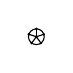
\begin{tikzpicture}[baseline=-0.5ex, scale=0.1]
    \draw (0,0) circle (1);
    \filldraw (0,0) circle (0.12);
    \foreach \angle in {90,162,234,306,378} {
      \draw (0,0) -- ({cos(\angle)}, {sin(\angle)});
      \filldraw ({cos(\angle)}, {sin(\angle)}) circle (0.08);
    }
  \end{tikzpicture}%
}
\title{\bfseries A note on optimal 2-planar graphs}
\author{Licheng Zhang, Yuanqiu Huang, Zhangdong Ouyang}
\date{Source: arXiv:2512.11535v3 (CC BY 4.0)}
\begin{document}
\maketitle

\noindent\emph{Source and licence.} \bfseries A note on optimal 2-planar graphs. Version arXiv:2512.11535v3 (CC BY 4.0), distributed by arXiv under the Creative Commons Attribution 4.0 International licence, http://creativecommons.org/licenses/by/4.0/, as recorded in the arXiv licence metadata for this exact version and shown on the abstract page https://arxiv.org/abs/2512.11535v3. Full licence notice: \texttt{licenses/arxiv-2512.11535-CC-BY-4.0.txt}.\par\smallskip

\noindent\textit{Editorial scope.} Counted unit: the article's lem lem:vertexFiveStar4-connected (source0.tex lines 458--461). The article's complete original proof of it is delivered with it (source0.tex lines 463--469, one \texttt{proof} environment of 7 lines). No mathematics is written, repaired or re-derived: the statement and the proof are the article's own lines, in the article's own notation, and no retained line is substituted or re-flowed.  Retained uncounted as the source-local context the proof needs: lines 284--286; lines 317--319.  Nothing was omitted from any retained span, so the package carries no omission record.  No retained line contains a citation, so the wrapper carries no bibliography and no bibliography entry.  No retained line contains a figure environment, an image-inclusion command or drawing code, so no image is delivered and the package declares no asset dependency.  Editorial formatting only, in addition: an AMS \texttt{amsart} preamble that restates the article's own declarations and macros used by the retained lines, namely the environments \texttt{prop}, \texttt{lem} on separate counters, together with the standard packages those lines need.  The retained environments print in this document as Proposition 1, Lemma 1 in order of appearance, whereas the article prints the same items with the numbering of its own full document.  The complete native source of the article as distributed in the arXiv e-print for this exact version is bundled unchanged as \texttt{sources/190879/source0.tex}.
\begin{prop}\label{prop:star-extension-4conn}
Let \(G\) be a \(3\)-connected plane graph. If \(g(G)\ge 4\), then \(G^{\vertexFiveStar}\) is \(4\)-connected.
\end{prop}

\begin{lem}\label{mainlem}
Let $G$ be a (simple) optimal 2-planar graph. Then $G$ has a 2-planar drawing obtained by drawing  a pentagram (that is, five mutually crossed edges) in the interior of each face of a 3-connected pentagulation.
\end{lem}

\begin{lem}\label{lem:vertexFiveStar4-connected}
Let \(G\) be an optimal \(2\)-planar graph with an op-drawing \(D\). 
If \(\kappa(G)\ge 4\), then \(P(D)^{\vertexFiveStar}\) is \(4\)-connected.
\end{lem}

\begin{proof}
By Lemma~\ref{mainlem}, \(P(D)\) is a \(3\)-connected pentagulation. 
We claim that \(P(D)\) has no separating \(3\)-cycle. 
Indeed, such a cycle would give a \(3\)-vertex-cut of \(G\), since its three uncrossed edges separate the vertices inside from those outside. 
Thus \(g(P(D))\ge 4\). 
The result now follows from Proposition~\ref{prop:star-extension-4conn}.
\end{proof}

\end{document}
